\documentclass[pdftex,12pt,a4paper,twoside,ngerman,numbers=noenddot]{scrbook}

% -------------------------------------------------------------------

% Seitenformat anpassen
\usepackage[a4paper,left=3.5cm,right=2.5cm,bottom=3.5cm,top=3cm]{geometry}
\setlength{\headheight}{19pt}

% -------------------------------------------------------------------

% Fix für alte Pakete mit KOMA Warnung
\usepackage{scrhack}

% -------------------------------------------------------------------

% Absolute Positionierung für Titelseite
\usepackage[absolute,overlay]{textpos}
\setlength{\TPHorizModule}{1mm}
\setlength{\TPVertModule}{\TPHorizModule}
\textblockorigin{0mm}{0mm}
\usepackage{setspace}

% -------------------------------------------------------------------

% Schrifteinstellungen
\usepackage{lmodern}
\usepackage[english,main=ngerman]{babel}
\usepackage[utf8]{inputenc}
\usepackage[T1]{fontenc}
\usepackage{ae,aecompl}

% -------------------------------------------------------------------

% Bibtex deutsch
\usepackage[numbers,sort]{natbib}

% -------------------------------------------------------------------

% Anführungszeichen
\usepackage[babel,german=quotes]{csquotes}

% -------------------------------------------------------------------

% URLs
\usepackage{url}

% Trennung langer URLs
\usepackage[hyphenbreaks]{breakurl}
\def\UrlBreaks{\do\a\do\b\do\c\do\d\do\e\do\f\do\g\do\h\do\i\do\j\do\k\do\l%
\do\m\do\n\do\o\do\p\do\q\do\r\do\s\do\t\do\u\do\v\do\w\do\x\do\y\do\z\do\0%
\do\1\do\2\do\3\do\4\do\5\do\6\do\7\do\8\do\9\do\-}%

% -------------------------------------------------------------------

% Caption anpassen
\usepackage[margin=0pt,font=small,labelfont=bf]{caption}

% -------------------------------------------------------------------

% Tabellen
\usepackage{booktabs}  % bessere Linien
\usepackage{siunitx}  % Ausrichtung von Dezimalstellen

% -------------------------------------------------------------------

% Zeilenabstand einstellen
\renewcommand{\baselinestretch}{1.25}

% Floating-Umgebungen anpassen
\renewcommand{\topfraction}{0.9}
\renewcommand{\bottomfraction}{0.8}

% -------------------------------------------------------------------

% Keine Einrücktiefe der ersten Zeile eines neuen Absatzes.
\parindent=0cm

% -------------------------------------------------------------------

% Kopfzeile hinzufügen
\usepackage[headsepline]{scrlayer-scrpage}
\clearpairofpagestyles{}

\lehead{\pagemark}
\rehead{\headmark}
\rohead{\pagemark}
\lohead{\headmark}

% -------------------------------------------------------------------

% Eigene Farben
\usepackage{xcolor}
\definecolor{TUGreen}{rgb}{0.517,0.721,0.094}
\definecolor{red}{rgb}{1,0,0}

% -------------------------------------------------------------------

% Algorithmen
\usepackage[plain,chapter]{algorithm}
\usepackage{algorithmic}

% Algorithmen anpassen
\renewcommand{\algorithmicrequire}{\textit{Eingabe:}}
\renewcommand{\algorithmicensure}{\textit{Ausgabe:}}
\floatname{algorithm}{Algorithmus}
\renewcommand{\listalgorithmname}{Algorithmenverzeichnis}
\renewcommand{\algorithmiccomment}[1]{\color{grau}{// #1}}

% -------------------------------------------------------------------

% Grafikpakete einbinden
\usepackage{graphicx}
\usepackage{subfigure}
\usepackage{pdfpages}
\usepackage{tikz}
\usetikzlibrary{decorations.pathreplacing}

% -------------------------------------------------------------------

% Mathematikpakete einbinden

\usepackage{amsmath,amssymb,amsthm}
\usepackage{mathtools}

% -------------------------------------------------------------------

% Todonotes einbinden

\usepackage{todonotes}

% -------------------------------------------------------------------

% Glossar
\usepackage[toc]{glossaries}
\glstoctrue{}
\makeglossaries{}
\newglossaryentry{N}{name=\ensuremath{\mathbb{N}}, description={Menge}}
\newglossaryentry{R}{name=\ensuremath{\mathbb{R}}, description={Menge der reellen Zahlen}}
\newglossaryentry{R+}{name=\ensuremath{\mathbb{R}^+}, description={Menge der positiven reellen Zahlen inklusive Null}}

\newglossaryentry{I}{name=\ma{I}, description={Identitätsmatrix}}

\newglossaryentry{diag}{name=\ensuremath{\mathrm{diag}}, description={Diagonalfunktion}}
\newglossaryentry{ortho}{name=\ensuremath{\perp}, description={Orthogonalität}}
\newglossaryentry{hadamard}{name=\ensuremath{\odot}, description={elementweises Hadamard-Produkt}}
\newglossaryentry{O}{name=\ensuremath{\mathcal{O}}, description={O-Notation}}
\newglossaryentry{T}{name=\ensuremath{T}, description={Tschebyschow-Polynom}}

\newglossaryentry{G}{name=\ensuremath{\mathcal{G}}, description={Graph}}
\newglossaryentry{V}{name=\ensuremath{\mathcal{V}}, description={Knotenmenge ${\left\{v_i\right\}}^N_{i=1}$ eines Graphen \gls{G}}}
\newglossaryentry{v}{name={\ensuremath{v}}, description={Knoten eines Graphen}}
\newglossaryentry{A}{name=\ma{A}, description={Adjazentmatrix eines Graphen \gls{G}}}
\newglossaryentry{D}{name=\ma{D}, description={gewichtete Gradmatrix}}
\newglossaryentry{L}{name=\ma{L}, description={Laplacian, unnormalisiert}}
\newglossaryentry{Lnorm}{name=\ma{\tilde{L}}, description={Laplacian, normalisiert}}
\newglossaryentry{Lboth}{name=\ma{\mathcal{L}}, description={Laplacian, normalisiert oder unnormalisiert}}
\newglossaryentry{w}{name=\ensuremath{w}, description={Gewichtsfunktion der Kanten eines Graph \gls{G} mit $\gls{w} \colon \gls{V} \times \gls{V} \to \gls{R+}$}}
\newglossaryentry{adj}{name=\ensuremath{\sim}, description={Adjazenzrelation zweiter Knoten eines Graphen \gls{G} mit $u \gls{adj} v$ genau dann, wenn $u$ und $v$ adjazent}}
\newglossaryentry{d}{name=\ensuremath{d}, description={gewichtete Gradfunktion der Knoten eines Graphen \gls{G} mit $\gls{d} \colon \gls{V} \to \gls{R+}$}}
\newglossaryentry{s}{name=\ensuremath{s}, description={kürzeste Pfaddistanz mit $s \colon \gls{V} \times \gls{V} \to \gls{N}$}}

\newglossaryentry{lambda}{name=\ensuremath{\lambda}, description={Eigenwert eines Eigenwertproblems $\ma{M}\ve{u} = \lambda\ve{u}$}}
\newglossaryentry{lambdamax}{name=\ensuremath{\lambda_{\max}}, description={Größter Eigenwert eines Eigenwertproblems $\ma{M}\ve{u} = \lambda\ve{u}$}}
\newglossaryentry{Lambda}{name=\ma{\Lambda}, description={Diagonalmatrix der Eigenwerte einer Matrix \ma{M} mit $\mathrm{diag}$}}
\newglossaryentry{eiv}{name=\ve{u}, description={normierter Eigenvektor zu einem Eigenwert mit $\left\|\gls{eiv}\right\|_2 = 1$}}
\newglossaryentry{Eiv}{name=\ma{U}, description={Eigenvektormatrix $\left[\ve{u}_1, \ldots, \ve{u}_N \right] \in \mathbb{R}^{N \times N}$ von $N$ Eigenvektoren $\ve{u}_i$}}
\newglossaryentry{Lambdatilde}{name=\ma{\tilde{\Lambda}}, description={reskalierte Diagonalmatrix der Eigenwerte des Laplacian}}
\newglossaryentry{Atilde}{name=\ma{\tilde{A}}, description={reskalierte Diagonalmatrix der Eigenwerte des Laplacian}}
\newglossaryentry{Dtilde}{name=\ma{\tilde{D}}, description={reskalierte Diagonalmatrix der Eigenwerte des Laplacian}}

\newacronym[plural=CNNs, longplural={Convolutional Neural Networks}]{CNN}{CNN}{Convolutional Neural Network}
\newacronym[plural=GCNs, longplural={Graph Convolutional Networks}]{GCN}{GCN}{Graph Convolutional Network}
\newacronym{SLIC}{SLIC}{Simple Linear Iterative Clustering}
\newacronym{MNIST}{MNIST}{Modified National Institute of Standards and Technology}
\newacronym{Cifar}{CIFAR}{Canadian Institute for Advanced Research}
\newacronym{Pascal}{PASCAL VOC}{Pascal Visual Object Classes}
\newacronym{SVHN}{SVHN}{Street View House Numbers}
\newacronym{PCA}{PCA}{Haptkomponentenanalyse}


% -------------------------------------------------------------------

% Fix für \left und \right Abstände
\let\oldleft\left
\let\oldright\right
\def\left#1{\mathopen{}\oldleft#1}
\def\right#1{\oldright#1\mathclose{}}

% -------------------------------------------------------------------

% Füge einen Punkt an Paragraph-Überschriften
\let\oldparagraph=\paragraph
\renewcommand\paragraph[1]{\oldparagraph{#1.}}

% -------------------------------------------------------------------

% Informationen für PDF-Dokument festlegen
\usepackage[pdfencoding=auto]{hyperref}

\hypersetup{pdfauthor={\Autor},
            pdftitle={\Titel},
            pdfsubject={\Arbeit, \Universitaet, \Fakultaet},
            pdfproducer={LaTeX},
            pdfview=FitV,
            pdfstartview=FitV,
            pdfhighlight=/I,
            pdfborder=0 0 0,
            colorlinks=false,
            bookmarksopen,
            bookmarksopenlevel=1,
            bookmarksnumbered=false,
            plainpages=false
}

\newglossaryentry{R}{name=\ensuremath{\mathbb{R}}, description={Menge der reellen Zahlen}}
\newglossaryentry{R+}{name=\ensuremath{\mathbb{R}_+}, description={Menge der positiven reellen Zahlen inklusive Null}}
\newglossaryentry{N}{name=\ensuremath{\mathbb{N}}, description={Menge der natürlichen Zahlen}}
\newglossaryentry{skalar}{name=\ensuremath{\left\langle \cdot, \cdot \right\rangle}, description={Skalarprodukt}}
\newglossaryentry{modulo}{name=\ensuremath{\text{mod}}, description={Modulo}}
\newglossaryentry{diag}{name=\ensuremath{\mathrm{diag}}, description={Diagonalfunktion}}
\newglossaryentry{I}{name=\ma{I}, description={Identitätsmatrix}}
\newglossaryentry{G}{name=\textcolor{red}{\ensuremath{G}}, description={Graph}}
\newglossaryentry{V}{name=\ensuremath{\mathcal{V}}, description={Knotenmenge ${\left\{v_i\right\}}^n_{i=1}$ eines Graphen \gls{G}}}
\newglossaryentry{E}{name=\ensuremath{\mathcal{E}}, description={Kantenmenge eines Graphen \gls{G} mit $\gls{E} \subseteq \gls{V} \times \gls{V}$}}
\newglossaryentry{adj}{name=\ensuremath{\sim}, description={Adjazenzrelation zweiter Knoten eines Graphen \gls{G} mit $u \gls{adj} v$ genau dann, wenn $u$ und $v$ adjazent}}
\newglossaryentry{w}{name=\ensuremath{w}, description={Gewichtsfunktion der Kanten eines Graph \gls{G} mit $\gls{w} \colon \gls{V} \times \gls{V} \to \gls{R+}$}}
\newglossaryentry{A}{name=\ma{A}, description={Adjazentmatrix eines Graphen \gls{G}}}
\newglossaryentry{Adist}{name=\ensuremath{\ma{A}_{\text{dist}}}, description={Distanzadjazentmatrix eines eingebetten Graphen \gls{G}}}
\newglossaryentry{Adistnorm}{name=\ensuremath{\ma{\tilde A}_{\text{dist}}}, description={normalisierte Distanzadjazentmatrix eines eingebetten Graphen \gls{G}}}
\newglossaryentry{Arad}{name=\ensuremath{\ma{A}_{\text{rad}}}, description={Winkeladjazentmatrix eines eingebetten Graphen \gls{G}}}
\newglossaryentry{F}{name=\ma{F}, description={Featurematrix eines Graphen}}
\newglossaryentry{Fout}{name=\ensuremath{\ma{F}^{\prime}}, description={Output-Featurematrix eines Graphen}}
\newglossaryentry{degree}{name=\ensuremath{\deg}, description={Gradfunktion der Knoten eines Graphen \gls{G} mit $\gls{degree} \colon \gls{V} \to \gls{N}$}}
\newglossaryentry{d}{name=\ensuremath{d}, description={gewichtete Gradfunktion der Knoten eines Graphen \gls{G} mit $\gls{d} \colon \gls{V} \to \gls{R+}$}}
\newglossaryentry{D}{name=\ma{D}, description={gewichtete Gradmatrix}}
\newglossaryentry{p}{name=\ensuremath{p}, description={Positionsfunktion auf den Knoten \gls{V} mit $\gls{p} \colon \gls{V} \to \gls{R}^2$}}
\newglossaryentry{s}{name=\ensuremath{s}, description={kürzeste Distanzfunktion mit $\gls{s} \colon \gls{V} \times \gls{V} \to \gls{N}$}}
\newglossaryentry{L}{name=\ma{L}, description={Laplacian, unnormalisiert}}
\newglossaryentry{Lnorm}{name=\ma{\tilde L}, description={Laplacian, normalisiert}}
\newglossaryentry{Lboth}{name=\ma{\mathcal{L}}, description={Laplacian, normalisiert oder unnormalisiert}}
\newglossaryentry{lambda}{name=\ensuremath{\lambda}, description={Eigenwert}}
\newglossaryentry{Lambda}{name=\ma{\Lambda}, description={Diagonalmatrix der Eigenwerte des Laplacian}}
\newglossaryentry{tLambda}{name=\ma{\tilde \Lambda}, description={reskalierte Diagonalmatrix der Eigenwerte des Laplacian}}
\newglossaryentry{tLboth}{name=\ensuremath{\mathcal{\tilde L}}, description={reskalierter Laplacian \gls{Lboth}}}
\newglossaryentry{ortho}{name=\ensuremath{\perp}, description={Orthogonalität}}
\newglossaryentry{eiv}{name=\ve{u}, description={Eigenvektor mit $\left\|\gls{eiv}\right\|_2 = 1$}}
\newglossaryentry{Eiv}{name=\ma{U}, description={Eigenvektormatrix}}
\newglossaryentry{hadamard}{name=\ensuremath{\odot}, description={Hadamard-Produkt}}
\newglossaryentry{T}{name=\ensuremath{T}, description={Tschebyschow-Polynom}}
\newglossaryentry{O}{name=\ensuremath{\mathcal{O}}, description={O-Notation}}
\newglossaryentry{a}{name=\ensuremath{a}, description={Voronoi-Gebiet über der Knotenmenge}}


\begin{document}

\selectlanguage{german}

% Titelseite
\begin{titlepage}

\definecolor{TUGreen}{rgb}{0.517,0.721,0.094}

\setlength{\TPHorizModule}{1cm}
\setlength{\TPVertModule}{1cm}
\setlength{\parindent}{0cm}

\sffamily

\vspace*{2cm}

\begin{textblock}{9}(3,5.3)
  \Large
  \begin{minipage}[c][9cm]{9cm}
    \begin{center}
      {\Huge Master-Thesis}\\
      \vspace*{1cm}
      {\huge Anwendbarkeit neuronaler Netze auf Graphrepräsentationen von Bildern}\\
      \vspace*{1cm}
      Matthias~Fey\\
      \today
    \end{center}
  \end{minipage}
  \normalsize
\end{textblock}

\begin{textblock}{9}(3,1)
  
\includegraphics[height=1.4cm]{images/tud_logo}
\end{textblock}

\begin{textblock}{15}(3,3.7)
  
\includegraphics[height=0.65cm]{images/fi_text}
\end{textblock}

\begin{textblock}{9}(3,26.5)
  
\includegraphics[height=1.2cm]{images/fi_logo}
\end{textblock}

\begin{textblock}{9}(3,20)
  \Large
  \textbf{Gutachter:}\\
  Prof.~Dr.~Heinrich~Müller\\
  M.Sc.~Jan~Eric~Lenssen
  \normalsize
\end{textblock}

\begin{textblock}{9}(3,24)
  \large
  \textcolor{TUGreen}{
    Lehrstuhl Informatik VII\\
    Graphische Systeme\\
    TU Dortmund
  }
  \normalsize
\end{textblock}

\end{titlepage}

\blankpage{}

% Inhaltsverzeichnis
\pagenumbering{roman}

\tableofcontents
\cleardoublepage{}

% Kapitel
\pagenumbering{arabic}

\chapter{Gedachter Inhalt}

\cite{Nielsen}
\cite{Dhillon}

Einleitung:
Motivation
Aufbau der Arbeit

Grundlagen:
Graphen, insbesondere planare Graphen
Mathematische Notationen: Vektor, Matrix, Tensor
Neuronale Netze (Was ist ein CNN, wie ist der Convolution Operator definiert, nicht lineare Aktivierungsfunktion)
Faltung, insbesondere Faltung im CNN

Graphrepräsentationen von Bildern
Grid
Superpixel
Superpixelalgorithmen
Umwandlung von Kanten von Distanz zu Gauß
Merkmalextraktion (Momente)
Merkmalselektion (Cov, PCA)

Lernen auf Graphen:
Stand der Forschung: Spatial vs Spectral

Spatial:
Patchy
Zentralität
Canonical Labeling
Übertragung auf planare Graphen <- EIGENER ANTEIL (z.B. Grid Spiral)
Komplexität
Vorteile (einfache Architektur)/Nachteile (keine direkte Nachbarschaftsberücksichtigung möglich,

keine Graph Coarsening möglich, Vorverarbeitung ist recht teuer und muss Preprocessed werden weil man das nicht über Matrixoperationen ausdrücken kann)

Spectral:
Laplacian, Fourier Transformation
GCN und kGCN (weisfeiler Lehman)
Übertragung auf planare Graphen (Adjazenzpartitionierung) <- EIGENER ANTEIL
Pooling/Coarsening
Komplexität
Vorteile (z.B. Nachbarschaftsberücksichtigung/keine Ordnung nötig)/Nachteile (rotationsinvariant)

Deep Learning auf variabler Input-Menge (SPP)

Augmentierung von Graphen (ist das überhaupt möglich)
COARSENING IST RANDOM (EINE FORM DER AUGMENTIERUNG)
PERMUTATE RANDOM
REMOVE RANDOM EDGE

Realisierung (Experimente) und Evaluation
Adam-Optimizer
Sparse Tensors
Vorstellung Datensätze (MNIST, PascalVOC, CIFAR-10, ImageNet)
Tensorflow
Dropout L2-Regularisierung

Zusammenfassung und Ausblick


\chapter{Einleitung}
\label{Einleitung}

\section{Motivation und Hintergrund}
\label{Motivation_und_Hintergrund}
%
Literatur~\cite{Abramowski:1991} oder~\cite{Abramowski:1991, Muller:2011} und Verweis auf Kapitel
\ref{Kapitel 2} ab Seite~\pageref{Kapitel 2}.

Homepage\footnote{\url{https://github.com/rusty1s/embedded\_gcnn}}

\section{Aufbau der Arbeit}
\label{Aufbau_der_Arbeit}

Er hörte \enquote{leise Schritte} hinter sich. Das bedeutete
nichts Gutes. Wer würde ihm schon folgen, spät in der Nacht und
dazu noch in dieser engen Gasse mitten im übel beleumundeten
Hafenviertel? Gerade jetzt, wo er das Ding seines Lebens gedreht
hatte und mit der Beute verschwinden wollte! Hatte einer seiner
zahllosen Kollegen dieselbe Idee gehabt, ihn beobachtet und
abgewartet, um ihn nun um die Früchte seiner Arbeit zu
erleichtern? Oder gehörten die Schritte hinter ihm zu einem der
unzähligen Gesetzeshüter dieser Stadt, und die stählerne Acht um
seine Handgelenke würde gleich zuschnappen? Er konnte die
Aufforderung stehen zu bleiben
schon hören.

Gehetzt sah er sich um. Plötzlich erblickte er den schmalen
Durchgang. Blitzartig drehte er sich nach rechts und verschwand
zwischen den beiden Gebäuden. Beinahe wäre er dabei über den
umgestürzten Mülleimer gefallen, der mitten im Weg lag. Er
versuchte, sich in der Dunkelheit seinen Weg zu ertasten und
erstarrte: Anscheinend gab es keinen anderen Ausweg aus diesem
kleinen Hof als den Durchgang, durch den er gekommen war. Die
Schritte wurden lauter und lauter, er sah eine dunkle Gestalt um
die Ecke biegen. Fieberhaft irrten seine Augen durch die
nächtliche Dunkelheit und suchten einen Ausweg. War jetzt wirklich
alles vorbei, waren alle Mühe und alle Vorbereitungen umsonst?

Er presste sich ganz eng an die Wand hinter ihm und hoffte, der
Verfolger würde ihn übersehen, als plötzlich neben ihm mit kaum
wahrnehmbarem Quietschen eine Tür im nächtlichen Wind hin und her
schwang. Könnte dieses der flehentlich herbeigesehnte Ausweg aus
seinem Dilemma sein? Langsam bewegte er sich auf die offene Tür
zu, immer dicht an die Mauer gepresst. Würde diese Tür seine
Rettung werden? Er hörte leise Schritte hinter sich. Das bedeutete
nichts Gutes. Wer würde ihm schon folgen, spät in der Nacht und
dazu noch in dieser engen Gasse mitten im übel beleumundeten
Hafenviertel? Gerade jetzt, wo er das Ding seines Lebens gedreht
hatte und mit der Beute verschwinden wollte! Hatte einer seiner
zahllosen Kollegen dieselbe Idee gehabt, ihn beobachtet und
abgewartet, um ihn nun um die Früchte seiner Arbeit zu
erleichtern? Oder gehörten die Schritte hinter ihm zu einem der
unzähligen Gesetzeshüter dieser Stadt, und die stählerne Acht um
seine Handgelenke würde gleich zuschnappen? Er konnte die
Aufforderung stehen zu bleiben schon hören. Gehetzt sah er sich
um. Plötzlich erblickte er den schmalen Durchgang. Blitzartig
drehte er sich nach rechts und verschwand zwischen den beiden
Gebäuden.

Er hörte \enquote{leise Schritte} hinter sich. Das bedeutete
nichts Gutes. Wer würde ihm schon folgen, spät in der Nacht und
dazu noch in dieser engen Gasse mitten im übel beleumundeten
Hafenviertel? Gerade jetzt, wo er das Ding seines Lebens gedreht
hatte und mit der Beute verschwinden wollte! Hatte einer seiner
zahllosen Kollegen dieselbe Idee gehabt, ihn beobachtet und
abgewartet, um ihn nun um die Früchte seiner Arbeit zu
erleichtern? Oder gehörten die Schritte hinter ihm zu einem der
unzähligen Gesetzeshüter dieser Stadt, und die stählerne Acht um
seine Handgelenke würde gleich zuschnappen? Er konnte die
Aufforderung stehen zu bleiben
schon hören.

Gehetzt sah er sich um. Plötzlich erblickte er den schmalen
Durchgang. Blitzartig drehte er sich nach rechts und verschwand
zwischen den beiden Gebäuden. Beinahe wäre er dabei über den
umgestürzten Mülleimer gefallen, der mitten im Weg lag. Er
versuchte, sich in der Dunkelheit seinen Weg zu ertasten und
erstarrte: Anscheinend gab es keinen anderen Ausweg aus diesem
kleinen Hof als den Durchgang, durch den er gekommen war. Die
Schritte wurden lauter und lauter, er sah eine dunkle Gestalt um
die Ecke biegen. Fieberhaft irrten seine Augen durch die
nächtliche Dunkelheit und suchten einen Ausweg. War jetzt wirklich
alles vorbei, waren alle Mühe und alle Vorbereitungen umsonst?


\section{Grundlagen}
\label{raeumliche_grundlagen}

Für die Definition eines räumlichen Faltungsoperators auf Graphen werden verschiedene Konstrukute der Graphentheorie benötigt.
Die


einer Abtastfolge \bzw{} einer Knotenauswahl sowie einer Nachbarschaftsgruppierung mit einer Ordnung
\todo{hier einleiten}

\paragraph{Färbung von Knoten}
\label{faerbung_von_knoten}

Eine \emph{Knotenfärbung} $\gls{l}$ ist eine nicht zwingend injektive Funktion $\gls{l} \colon \gls{V} \to \gls{C}$ auf den Knoten eines Graphen \gls{G}, die jedem Knoten in \gls{V} eine \emph{Farbe} einer endlich abzählbaren Menge $\gls{C} \subseteq \gls{R}$ zuordnet~\cite{patchy}.
Mit Hilfe der Knotenfärbung lässt sich folglich eine Ordungsrelation $>_{\gls{l}}$ auf der Knotenmenge von \gls{G} definieren, wobei $\gls{v}_i >_{\gls{l}} \gls{v}_j$ genau dann, wenn $\gls{l}\left(\gls{v}_i\right) < \gls{l}\left(\gls{v}_j\right)$~\cite{patchy}.
Falls \gls{l} weiterhin injektiv ist, so spricht man von einer \emph{totalen Ordnung} und die Knoten $\gls{v} \in \gls{V}$ können insbesondere so permutiert werden, dass sie die Ordnung von $>_{\gls{l}}$ respektieren~\cite{patchy}.

Beispiele für eine Knotenfärbung sind Metriken, die die Wichtigkeit der einzelnen Knoten beschreiben.
Eine naive Metrik dafür ist \zB{} der Knotengrad \gls{degree} \bzw{} \gls{d}, der die \emph{Zentralität} der Knoten beschreibt~\cite{patchy}.
Komplexere Metriken für die Zentralität der Knoten sind unter anderem die Nähe, die Betweenness-Zentralität sowie die Eigenvektorzentralität~\cite{patchy, centrality}.
Letztere ist eng mit dem \emph{PageRank}-Algorithmus von Google verwandt ist~\cite{centrality}.
Die \emph{Nähe} (\engl{} \emph{Closeness})
\begin{equation*}
  c\left(\gls{v}\right) \coloneqq \frac{1}{\sum_{\gls{v}_i \in \gls{V}, \gls{v} \neq \gls{v}_i} \gls{s}\left(\gls{v}, \gls{v}_i\right)}
\end{equation*}
ist ein Maß für die durchschnittliche Länge zwischen einem Knoten und allen weiteren Knoten in \gls{V}~\cite{centrality}.
Je \emph{näher} ein Knoten sich an der Knotenmenge befindet, als desto zentraler gilt er.
Die \emph{Betweeness-Zentralität} eines Knotens $\gls{v} \in \gls{V}$ ist über
\begin{equation*}
  c\left(\gls{v}\right) \coloneqq \sum_{\gls{v}_i \neq \gls{v} \neq \gls{v}_j} \frac{\kappa_{ij}\left(\gls{v}\right)}{\kappa_{ij}}
\end{equation*}
definiert, wobei $\kappa_{ij} \in \gls{N}$ die Anzahl an kürzesten Pfaden von $\gls{v}_i$ nach $\gls{v}_j$ angibt und $\kappa_{ij}\left(\gls{v}\right) \in \gls{N}$ die Anzahl dieser Pfade beschreibt, die durch \gls{v} führen~\cite{centrality}.
Nach der Methode der \emph{Eigenvektorzentralität} gilt ein Knoten als umso wichtiger, je wichtiger seine Nachbarknoten sind~\cite{centrality}.
Sie ist definiert über
\begin{equation*}
  c\left(\gls{v}\right) = \frac{1}{\gls{lambda}} \sum_{\gls{v}_i \in \gls{Neighbor}\left(\gls{v}\right)} c\left(\gls{v}_i\right),
\end{equation*}
wobei $\gls{lambda} \in \gls{R}$.
Mit der Darstellung der Eigenvektorzentralität $c \colon \gls{V} \to \gls{R+}$ als Vektor $\ve{c} \in \gls{R+}^N$ und \gls{G} als ungewichtete Adjazenzmatrix $\gls{A} \in {\left\{0,1\right\}}^{N \times N}$ kann die Bestimmung von \gls{lambda} \bzw{} \ve{c} als Eigenwertproblem $\gls{A}\ve{c} = \gls{lambda}\ve{c}$ aufgefasst werden.
Dann beschreibt der größte Eigenwert \gls{lambda} die Eigenvektorzentralität der Knoten über dessen Eigenvektor \ve{c}~\cite{centrality}.

\paragraph{Isomorphie und kanonische Ordnung}
\label{isomorphie_und_kanonische_ordnung}

Seien $\gls{G}_1 = \left(\gls{V}_1, \gls{E}_1\right)$ und $\gls{G}_2 = \left(\gls{V}_2, \gls{E}_2\right)$ zwei Graphen mit der gleichen Anzahl an Knoten, \dhe{} $\left|\gls{V}_1\right| = \left|\gls{V}_2\right|$.
Dann heißt eine bijektive Abbildung $p \colon \gls{V}_1 \to \gls{V}_2$ \emph{Isomorphismus} zwichen $\gls{G}_1$ und $\gls{G}_2$, falls $\left(\gls{v}_i, \gls{v}_j\right) \in \gls{E}_1$ \gdw{} $\left(p\left(\gls{v}_i\right), p\left(\gls{v}_j\right)\right) \in \gls{E}_2$~\cite{nauty}.
Zwei Graphen sind \emph{isomorph} zueinander, falls ein Isomorphismus zwischen ihnen existiert.
Die Komplexität zur Bestimmung der Isomorphie zweier Graphen liegt in NP, wobei nicht bekannt ist, ob sie in P enthalten oder NP-vollständig ist~\cite{patchy}.

Die Komposition mehrerer Isomorphismen ist ebenfalls ein Isomorphismus~\cite{nauty}.
Die Menge aller Isomorphismen (zuzüglich der identischen Abbildung, die die Knoten auf sich selber abbildet) heißt die \emph{Isomorphismenklasse} des Graphen~\cite{nauty}.

Eine \emph{kanonische Ordnung} eines Graphen $\gls{G} = \left(\gls{V}, \gls{E}\right)$ ist ein Graph $\gls{G}^{\prime} = \left(\gls{V}^{\prime}, \gls{E}^{\prime}\right)$ mit einer eindeutigen Ordnung seiner Knoten $\gls{V}^{\prime}$, der isomorph zu \gls{G} ist und seine gesamte Isomorphismenklasse repräsentiert~\cite{patchy}.
Zwei Graphen sind insbesondere genau dann zueinander isomorph, wenn ihre kanonischen Ordnungen übereinstimmen~\cite{nauty}.
Abbildung~\ref{fig:kanonische_ordnung} illustriert das Prinzip einer kanonischen Ordnung anhand zwei einfach gewählter isomorpher Graphen.
\begin{figure}[t]
\centering
\begin{tikzpicture}
  \tikzstyle{node}=[circle,draw, minimum width=18pt, inner sep=0pt, fill=white]

  \node[node] (a1) at (0, 4) {$8$};
  \node[node] (a2) at (1, 4) {$3$};
  \node[node] (a3) at (2, 4) {$2$};
  \node[node] (a4) at (3, 4) {$7$};
  \node[node] (a5) at (0, 3) {$5$};
  \node[node] (a6) at (1, 3) {$1$};
  \node[node] (a7) at (2, 3) {$6$};
  \node[node] (a8) at (3, 3) {$4$};

  \path (a1) edge (a2);
  \path (a1) edge (a5);
  \path (a2) edge (a3);
  \path (a2) edge (a6);
  \path (a2) edge (a7);
  \path (a3) edge (a4);
  \path (a3) edge (a6);
  \path (a3) edge (a7);
  \path (a4) edge (a8);
  \path (a5) edge (a6);
  \path (a6) edge (a7);
  \path (a7) edge (a8);

  \node[node] (b1) at (0, 1) {$4$};
  \node[node] (b2) at (1, 1) {$8$};
  \node[node] (b3) at (2, 1) {$6$};
  \node[node] (b4) at (3, 1) {$2$};
  \node[node] (b5) at (0, 0) {$3$};
  \node[node] (b6) at (1, 0) {$7$};
  \node[node] (b7) at (2, 0) {$5$};
  \node[node] (b8) at (3, 0) {$1$};

  \path (b1) edge (b2);
  \path (b1) edge (b5);
  \path (b2) edge (b3);
  \path (b2) edge (b6);
  \path (b2) edge (b7);
  \path (b3) edge (b4);
  \path (b3) edge (b6);
  \path (b3) edge (b7);
  \path (b4) edge (b8);
  \path (b5) edge (b6);
  \path (b6) edge (b7);
  \path (b7) edge (b8);

  \node[node] (c1) at (8,  4) {$6$};
  \node[node] (c2) at (9,  4) {$4$};
  \node[node] (c3) at (10, 4) {$2$};
  \node[node] (c4) at (11, 4) {$1$};
  \node[node] (c5) at (8,  3) {$5$};
  \node[node] (c6) at (9,  3) {$3$};
  \node[node] (c7) at (10, 3) {$7$};
  \node[node] (c8) at (11, 3) {$8$};

  \path (c1) edge (c2);
  \path (c1) edge (c5);
  \path (c2) edge (c3);
  \path (c2) edge (c6);
  \path (c2) edge (c7);
  \path (c3) edge (c4);
  \path (c3) edge (c6);
  \path (c3) edge (c7);
  \path (c4) edge (c8);
  \path (c5) edge (c6);
  \path (c6) edge (c7);
  \path (c7) edge (c8);

  \node[node] (d1) at (8,  1) {$4$};
  \node[node] (d2) at (9,  1) {$8$};
  \node[node] (d3) at (10, 1) {$5$};
  \node[node] (d4) at (11, 1) {$1$};
  \node[node] (d5) at (8,  0) {$3$};
  \node[node] (d6) at (9,  0) {$7$};
  \node[node] (d7) at (10, 0) {$6$};
  \node[node] (d8) at (11, 0) {$2$};

  \path (d1) edge (d2);
  \path (d1) edge (d5);
  \path (d2) edge (d3);
  \path (d2) edge (d6);
  \path (d2) edge (d7);
  \path (d3) edge (d4);
  \path (d3) edge (d6);
  \path (d3) edge (d7);
  \path (d4) edge (d8);
  \path (d5) edge (d6);
  \path (d6) edge (d7);
  \path (d7) edge (d8);

  \draw[<->] (4,   3.5) -- node[above] {unterschiedlich}          (7,   3.5);
  \draw[<->] (4,   0.5) -- node[above] {identisch}                (7,   0.5);
  \draw[->]  (1.5, 2.5) -- node[right] {kanonisiere~\cite{nauty}} (1.5, 1.5);
  \draw[->]  (9.5, 2.5) -- node[left]  {kanonisiere~\cite{nauty}} (9.5, 1.5);

\end{tikzpicture}
\caption[Kanonische Ordnung]{Illustration zweier isomorpher Graphen (oben), die jedoch nicht identisch sind (\zB{} sind die Knoten $1$ und $5$ im linken Graphen adjazent, aber nicht im rechten).
Der Prozess zur Bestimmung einer kanonischen Ordnung sorgt dafür, dass zwei Graphen eine identische Knotenabbildung erhalten, falls sie isomorph zueinander sind (unten).
Die Kanten der Graphen verweisen jeweils auf die gleichen Indizes, auch wenn sich die Darstellung \bzw{} Position der Knoten unterscheidet.}
\label{fig:kanonische_ordnung}
\end{figure}


Ein Isomorphismus \bzw{} eine kanonische Ordnung kann ebenfalls eine Knotenfärbung \gls{l} berücksichtigen, indem Knoten durch einen Isomorphismus nur auf Knoten der gleichen Farbe abgebildet werden dürfen~\cite{nauty}.
Das reduziert die Menge der verfügbaren Isomorphismenklassen und insbesondere die Komplexität ihrer Berechnung.
Zur Berechnung der Isomorphismenklassen und der kanonischen Ordnung, auch unter Berücksichtigung einer Knotenfärbung, zeichnet sich das Programm \texttt{nauty} aufgrund dessen bemerkenswerter Berechnungslaufzeit aus (\vgl{}~\cite{nauty}).


\chapter{Graphrepräsentationen von Bildern}

planarer Graph (MUSS NICHT UNBEDINGT SEIN), gegenbeispiel, ist aber auch egal


\chapter{Räumliche Graphentheorie}

Isomorphismus, Automorphismus, Canonical Labeling

Labeling / Node Partitions

\section{Patchy-SAN}


\chapter{Spektrale Graphentheorie}

\begin{itemize}
  \item \emph{Spektrum} eines Graphen zur Untersuchung seiner Eigenschaften
  \item \emph{algebraische} oder \emph{spektrale Graphentheorie} genannt
  \item als Spektrum eines Graphen bezeichnet man die (nach Größe geordnete) Folge der Eigenwerte $\lambda$ seiner Adjazenzmatrix, d.h. $A \cdot x = \lambda x$ ($x$ Eigenvektoren)
\end{itemize}

Algebraische Methoden sind sehr effektiv bei Graphen, die regulär und symmetrisch sind.
Als \emph{Schleife} wird in der Graphentheorie eine Kante bezeichnet, die einen Knoten mit sich selbst verbindet.
Ein Graph ohne Schleifen wird \emph{schleifenloser} Graph genannt.

Sei $d_v$ der Grad eines Knotens $v$ eines Graphen $G$.
Der \emph{Laplacian} $\mathcal{L}$ eines Graphen ohne Schleifen und Mehrfachkanten ist definiert als

\begin{equation}
  \mathcal{L}(u, v) = \begin{cases}
    d_v, & \text{wenn }u = v\text{,}\\
    -1, & \text{wenn }u\text\ {und }v\ \text{adjazent,}\\
    0, & \text{sonst.}
  \end{cases}
\end{equation}

Der Graph Laplacian ist eine Generalisierung des Laplacian auf einem Gitter.

Damit ist $\mathcal{L} = D - A$.
$\mathcal{L}$ kann normalisiert werden über $\mathcal{L}_{\text{norm}} = T^{-\frac{1}{2}}LT^{-\frac{1}{2}}$, wobei $T$ die Diagonalmatrix beschreibt mit $T(v, v) = d_v$.
Für einen \emph{isolierten} Knoten $v$, d.h.\ $d_v = 0$, gilt die Konvention $T^{-1}(v, v) = 0$.
Ebenso lässt sich $\mathcal{L}_{\text{norm}}$ definieren als

\begin{equation}
  \mathcal{L}_{\text{norm}}(u, v) = \begin{cases}
    1, & \text{wenn }u = v\text{und }d_v \neq 0\text{,}\\
    -\frac{1}{\sqrt{d_u d_v}}, & \text{wenn }u\text\ {und }v\ \text{adjazent,}\\
    0, & \text{sonst.}
  \end{cases}
\end{equation}

Der normalisierte Laplacian ist immer noch symmtrisch!

Wenn $G$ $k$-regulär ist, d.h.\ $T = \text{diag}(k)$, dann gilt $\mathcal{L}_{\text{norm}} = I - \frac{1}{k}A$.

Da $\mathcal{L}$ symmetrisch ist, sind seine Eigenwerte alle $\geq 0$ (d.h. $\mathcal{L}$ ist positiv-semidefinit).
Jede Reihen- und Spaltensumme von $\mathcal{L}$ ist $0$.

Einem gewichtetem ungerichterem Graph $G$ kann eine Gewichtsfunktion $w: V \times V \rightarrow \mathbb{R}$ zugeschrieben werden, sodass $w(u, v) = w(v, u)$ und $w(u, v) \geq 0$.
Falls $\lbrace u, v \rbrace \notin \mathcal{E}$, dann $w(u, v) = 0$.
Damit sind ungewichtete Graphen nur ein Spezialfall bei dem alle Gewichte $0$ oder $1$ sind.
Der Grad $d_v$ eines Knoten $v$ ist dann definiert als

\begin{equation}
  d_v = \sum_u w(u, v).
\end{equation}

Dann gilt

\begin{equation}
  \mathcal{L} = \begin{cases}
    1 - \frac{w(v, v)}{d_v}, & \text{wenn }u = v\text{und }d_v \neq 0\text{,}\\
    -\frac{w(u,v)}{\sqrt{d_u d_v}}, & \text{wenn }u\text\ {und }v\ \text{adjazent,}\\
    0, & \text{sonst.}
  \end{cases}
\end{equation}

Bemerke, dass hier Schleifen nicht explizit ausgeschlossen werden!

Eine Verschrumpfung eines Graphen $G$ kann beschrieben werden über zwei verschiedene Knoten $u$ und $v$ zu einem neuen Knoten $v^*$ mit

\begin{equation}
  w(x,v^*) = w(x, u) + w(x, v)
\end{equation}

und

\begin{equation}
  w(v^*, v^*) = w(u, u) + w(v, v) + 2w(u,v)
\end{equation}

Mit $\lambda_G := \lambda_1$ für einen Graphen $G$, gilt für einen Graphen $H$ der aus $G$ verkleinert wurde

\begin{equation}
  \lambda_G \leq \lambda_H
\end{equation}

\section{Spectral Graph Domain}

\begin{itemize}
  \item \emph{Spectral Graph Domain}: Der Raum der Eigenfunktionen von $\mathcal{L}$
  \item Analogon (Nachbildung) einer \emph{Fourier-Transformation} von Funktionen auf gewichteten Graphen
\end{itemize}

Eine beliebige Funktion $f: V \rightarrow \mathbb{R}$ kann als ein Vektor in $\mathbb{R}^n$ gesehen werden.
Dies impliziert eine Ordnung auf den Knoten.
Wir schreiben $f \in \mathbb{R}^n$ für Funktionen auf den Knoten eines Graphen und $f(m)$ für den Wert des $m$ten Knoten.

Dann gilt für eine beliebige Funktion $f \in \mathbb{R}^n$

\begin{equation}
  \mathcal{L}f(x) = \sum_{x~y} w(x, y) \cdot (f(x) - f(y))
\end{equation}

wobei die Summe über $x~y$ die Summierung über alle Knoten $y$ beschreibt, die adjazent zu $x$ sind.

Angenommen $G$ ist als ein reguläres Gitter definiert der Breite und Höhe $M$
Dann hat ein Knoten $v_{x,y}$ genau 4 Nachbarn mit Kantengewicht $\frac{1}{{(\delta w)}^2}$, bei dem $\delta w$ die euklidsche Distanz zwischen zwei Gitterpunkten beschreibt.

Für eine Funktion $f: M \times M \rightarrow \mathbb{R}$ gilt dann:

\begin{equation}
  \mathcal{L}f(x, y) = \frac{4f(x,y) - f(x+1, y) - f(x-1, y) - f(x, y+1) - f(x, y-1)}{{(\delta w)}^2}
\end{equation}

Damit kann ein Signal $f$ mit der Multiplikation mit $\mathcal{L}$ als eine Weiterpropagation von $f$ unter der Berücksichtigung der lokalen Nachbarn verstanden werden (\emph{5-point Stencil}, d.h.\ $\mathcal{L}f \approx - \nabla^2 f$).

\section{Diskrete Fourier Transformation}

$\mathcal{L}$ besitzt genau $n$ orthogonal zueinander stehende Eigenvektoren $\lbrace u_l \rbrace_{l=1}^n \in \mathbb{R}^n$.
Eigenvektoren $u_i$ sind auf $1$ normiert, d.h.\ $||u_i||_2 = 1$.
Diese werden auch \emph{Graph Fourier Modes} genannt.
Diesen sind Eigenwete $\lbrace \lambda_l \rbrace_{l=1}^n \in \mathbb{R}$ zugeordnet, die die \glqq{}Frequenzen\grqq\ bzw.\ das Spektrum des Graphen beschreiben oder visuell betrachtet die Ausdehnung des Raumes, den die Eigenvektoren aufspannen.
Bemerke dass $\lambda_0 = 0$, da für den Eigenvektor $\vec{u_0} = {(1, 1, \ldots, 1)}^T$ gilt, dass $\mathcal{L}\vec{u_0} = 0$.
$\mathcal{L}$ ist diagonalisierbar über $\mathcal{L} = U \Lambda U^T$, wobei $U = [u_1, \ldots, u_n] \in \mathbb{R}^{n \times n}$ die \emph{Fourier Basis} und $\Lambda = \text{diag}([\lambda_0, \ldots, \lambda_n]) \in \mathbb{R}^{n \times n}$.
Die \emph{Fourier Transformation} eines Signals $x \in \mathbb{R}^n$ ist dann definiert als $\hat{x} = U^{T}x$ und die Inverse als $x = U\hat{x}$.

\section{Faltung}

Wir suchen einen Operator $x *_G g$, der eine Faltung zweier Eingangssignale $x, g$ zu einem Ausgangssignal umleitet.
$x$ beschreibt dabei die Knotenattribute und $g$ die Gewichte.

\subsection{Faltung in CNNs}

In der Funktionalanalysis beschreibt die \emph{Faltung} einen mathematischen Operator, der für zwei Funktion $f$ und $g$ eine dirtte Funktion $f * g$ liefert.
Die Faltung kann als ein Produkt von Funktionen vertanden werden.

Anschaulich ist $(f * g)(x)$ der \emph{gewichtete Mittelwert} von $f$, wobei die Gewichtung durch $g$ gegeben ist.

Angenommen wir wollen über einer Matrix mit einem \emph{Filter} falten.
Sei unsere Eingangsmatrix $3 \times 4$ und unsere Filtergröße $2 \times 2$.

Dann gilt zum Beispiel für den Faltungsoperator $*$ in einem Convolutional Neural Network:

\begin{equation}
  \begin{pmatrix}
    1 & 2 & 3 & 1\\
    4 & 5 & 6 & 1\\
    7 & 8 & 9 & 1
  \end{pmatrix} * \begin{pmatrix}
    1 & 1\\
    1 & 1
  \end{pmatrix} = \begin{pmatrix}
    12 & 16 & 11\\
    24 & 28 & 17
  \end{pmatrix}
\end{equation}

$f: 3 \times 4 \rightarrow \mathbb{R}$ und $g: 2 \ times 2 \rightarrow \mathbb{R}$, dann ist $*$ definiert als

\begin{equation}
  (f * g)(x, y) = \sum_{x_i \in [x, x+1]\\y_i \in [y, y+1]} f(x_i, y_i)g(x-x_i, y-y_i)
\end{equation}

\subsection{Faltung auf Graphen}

Da wir keinen Translationsoperator auf der Domäne der Knoten $x$ beschreiben können, müssen wir unseren Faltungsoperator in der Fourier-Domäne beschreiben.
Dafür wandeln wir unsere Knotenmenge $x$ zuerst in $\hat x$ um.

Wir definieren $*_G$ in der Fouier-Domäne als

\begin{equation}
  x *_G g = U \cdot (U^T \cdot x \odot \hat g)
\end{equation}

wobei $\odot(A, B) = (a_{ij} \cdot b_{ij})$ die elementweise Multiplikation bzw.\ das \emph{Hadamard-Produkt}.

Das Hadamard-Produkt löst sich auf, wenn $\hat g$ als eine Diagonalmatrix repräsentiert wird. Dann gilt

\begin{equation}
  x *_G g = U \begin{pmatrix}
    \hat g(\lambda_0) & \cdots & 0\\
    0 & \cdots & \hat g(\lambda_n)
  \end{pmatrix}U^T x = U \hat g(\Lambda) U^T x
\end{equation}

Dann beschreibt $\hat g(\Lambda) = \text{diag}(\theta)$ eine Gewichtsfunktion mit $n$ Variablen, $\theta \in \mathbb{R}^n$.
Damit ist die Faltung bzw.\ die Gewichtung abhängig von der Input-Größe $n$, was extrem schlecht ist.

\subsection{Offene Fragen}

\begin{itemize}
  \item Wie erklärt sich noch einmal der normalisierte Laplacian?
  \item Warum wird $\hat g$ als Diagonalmatrix repräsentiert?
  \item Wie kommt die Convolution zustande mit dem $*$ Operator?
  \item Was passiert bei gerichteten Graphen???? Wir haben keinen symmetrischen und insbesondere keinen positiv definiten
\end{itemize}

\subsection{Beispiel}

Wir betrachten eine einfache $3 \times 3$ Adjazenzmatrix, d.h.\ $|\mathcal{V}| = n = 3$.

\begin{equation}
  A = \begin{pmatrix}
    0 & 1 & 0\\
    1 & 0 & 1\\
    0 & 1 & 0
  \end{pmatrix}
\end{equation}

mit Diagonalmatrix $D = \text{diag}(1, 2, 1)$.

Der Laplacian $\mathcal{L} = D - A$ ist dann

\begin{equation}
  \mathcal{L} = \begin{pmatrix}
    1 & -1 & 0\\
    -1 & 2 & -1\\
    0 & -1 & 1
  \end{pmatrix}
\end{equation}

Nun müssen die Eigenvektoren der Matrix und dessen Eigenwerte bestimmt werden, d.h.\ wir müssen das folgende Eigenwertproblem lösen

\begin{equation}
  \mathcal{L} \cdot \vec{u} = \lambda \cdot \vec{u}
\end{equation}

Wir erhalten $3$ Eigenvektoren und Eigenwerte mit

\begin{equation}
  \lambda_0 = 0, \vec{u}_0 = \frac{1}{\sqrt{3}} \begin{pmatrix}1\\1\\1\end{pmatrix} \approx \begin{pmatrix}0.58\\0.58\\0.58\end{pmatrix},
    \lambda_1 = 1, \vec{u}_1 = \frac{1}{\sqrt{2}} \begin{pmatrix}-1\\0\\1\end{pmatrix} \approx \begin{pmatrix}-0.71\\0\\0.71\end{pmatrix},
      \lambda_2 = 3, \vec{u}_2 = \frac{1}{\sqrt{6}} \begin{pmatrix}1\\-2\\1\end{pmatrix} \approx \begin{pmatrix}0.41\\-0.82\\0.41\end{pmatrix}
\end{equation}

Dann sind $U$, $\Lambda$ und $U^T$ definiert als

\begin{equation}
  U \approx \begin{pmatrix}
    0.58 & -0.71 & 0.41\\
    0.58 & 0 & -0.82\\
    0.58 & 0.71 & 0.41
  \end{pmatrix},
  \Lambda = \begin{pmatrix}
    0 & 0 & 0\\
    0 & 1 & 0\\
    0 & 0 & 3
  \end{pmatrix},
  U^T \approx \begin{pmatrix}
    0.58 & 0.58 & 0.58\\
    -0.71 & 0 & 0.71\\
    0.41 & -0.82 & 0.41
  \end{pmatrix}
\end{equation}

Angenommen wir haben ein Signal $x = {(100, 10, 1)}^T$, dann ist der Wert dieses Signals transformiert in die Fourier Domäne definiert als $\hat x \approx {(64.09, -70.00, 33.07)}^T$.
Führen wir $\hat x$ auf $x$ mittels $U \cdot \hat x$ zurück, erhalten wir korrekterweise $x = {(100, 10, 1)}^T$.

Ich habe absolut keine Ahnung was diese Sachen aussagen sollen :D:D

\section{Chebyshev Polynome}

\section{Probleme}

Rotationsinvariant

\section{Pfadlänge}

wenn $d_G(m,n) > k$, dann ${(L^k)}_{m, n} = 0$
(normalisiert sowie unnormalisiert (siehe Wavelet Lemma 5.4))

\section{Graph Convolutional Networks}
\label{graph_convolutional_networks}

\citeauthor{gcn} motivieren einen weiteren Ansatz zur Faltung auf Graphen, genannt \emph{\gls{GCN}}, der auf der Methodik des spekralen Faltungsoperators aus Kapitel~\ref{spektraler_faltungsoperator} aufbaut und dabei wie eine \enquote{differenzierbare und parametrisierte Generalisierung des eindimensionalen Weisfeiler-Lehman Algorithmus auf Graphen} fungiert~\cite{gcn}.

\paragraph{Faltungsoperator}
\label{gcn_faltungsoperator}

Sei $\ve{f}_{\mathrm{in}} \star \ve{\hat g} \approx \sum_{k=0}^K c_k \gls{T}_k\left(\gls{Lbothtilde}\right) \ve{f}_{\mathrm{in}}$ der in~\eqref{eq:tschebyschow_faltung_L} definierte spektrale Faltungsoperator mit $K=1$.
Dann ist $\ve{f}_{\mathrm{in}} \star \ve{\hat g}$ eine lineare Funktion \bzgl{} \gls{Lboth} und damit eine lineare Funktion auf dem Spektrum des Graphen~\cite{gcn}.
Mit $K=1$ betrachtet der spektrale Faltungsoperator nur noch die lokale Nachbarschaft eines jeden Knotens (\vgl{}~\ref{polynomielle_approximation}).
Es ist anzumerken, dass dies in der Regel keinen Nachteil darstellt.
So hat es sich bei gegenwärtigen \enquote{State-of-the-Art}-\glspl{CNN} auf Bildern ebenfalls eingebürgert, nur noch über minimale $3\times3$ Filtergrößen zu falten und stattdessen Merkmale weit entfernterer Knoten über die mehrfache Aneinanderreihung der Faltungsschichten mittels tieferer Netze zu gewinnen~(\vgl{}~\cite{gcn, vgg, He}).
Unter dieser Restriktion vereinfacht sich $\ve{f}_{\mathrm{in}} \star \ve{\hat g}$ zu
\begin{equation}
  \ve{f}_{\mathrm{in}} \star \ve{\hat g} \approx c_0\, \ve{f}_{\mathrm{in}} + c_1 \left(\frac{2}{\gls{lambdamax}}\gls{Lboth} - \gls{I}\right)\ve{f}_{\mathrm{in}}
  \label{eq:gcn_faltung_both}
\end{equation}
mit zwei freien Parametern $c_0$ und $c_1$~\cite{gcn}.
Für $\gls{Lnorm}$ auf einem zusammenhängenden Graphen \gls{G} gilt dann nach~\eqref{eq:gcn_faltung_both} weiter
\begin{equation}
  \ve{f}_{\mathrm{in}} \star \ve{\hat g} \approx c_0 \, \ve{f}_{\mathrm{in}} + c_1 \left(\gls{Lnorm} - \gls{I}\right)\ve{f}_{\mathrm{in}} = c_0 \, \ve{f}_{\mathrm{in}} - c_1 \gls{D}^{-\frac{1}{2}} \gls{A} \gls{D}^{-\frac{1}{2}} \ve{f}_{\mathrm{in}},
  \label{eq:gcn_faltung_norm}
\end{equation}
wobei $\gls{lambdamax} \coloneqq 2$ auf dessen obere Schranke gesetzt wird~\cite{gcn}.
Um die Gefahr des Overfittings und die Anzahl an Berechnungen pro Schicht weiter zu beschränken, reduziert sich~\eqref{eq:gcn_faltung_norm} mit einem einzigen Parameter $c \coloneqq c_0$ mit $c = -c_1$ zu~\cite{gcn}
\begin{equation*}
  \ve{f}_{\mathrm{in}} \star \ve{\hat g} \approx c \left(\gls{I} + \gls{D}^{-\frac{1}{2}} \gls{A} \gls{D}^{-\frac{1}{2}} \right) \ve{f}_{\mathrm{in}}.
\end{equation*}
Die skalierten Eigenwerte von \gls{Lambdatilde} liegen auf Grund der Addition mit \gls{I} nun im Intervall $\left[0, 2\right]$ (\vgl{}~\cite{gcn}).
Demnach können wiederholte Anwendungen des Faltungsoperators zu \enquote{numerischen Instabilitäten und folglich zu explodierenden oder verschwindenen Gradienten} führen~\cite{gcn}.
\citeauthor{gcn} führen zur Behebung dieses Problems die folgende Renormalisierung durch: $\gls{I} + \gls{D}^{-1/2} \gls{A} \gls{D}^{-1/2} \rightarrow \gls{Dtilde}^{-1/2} \gls{Atilde} \gls{Dtilde}^{-1/2}$ mit $\gls{Atilde} \coloneqq \gls{A} + \gls{I}$ und $\gls{Dtilde}_{ii} \coloneqq \sum_{j=1}^N \gls{Atilde}_{ij}$.
Der entgültige Faltungsoperator des \glspl{GCN} ergibt sich dann als
\begin{equation}
  \ve{f}_{\mathrm{in}} \star \ve{\hat g} \approx c\, \gls{Dtilde}^{-\frac{1}{2}} \gls{Atilde} \gls{Dtilde}^{-\frac{1}{2}} \ve{f}_{\mathrm{in}}
  \label{eq:gcn_renorm}
\end{equation}
auf einem einzigen freien Parameter $c \in \gls{R}$.

\paragraph{Implementierung}
\label{gcn_tensor}

Die Faltung des \glspl{GCN} auf Merkmalsmatrizen lässt sich analog zur Tensorimplementierung des spektralen Faltungsoperators in Kapitel~\ref{polynomielle_approximation} beschreiben, mit dem Unterschied, dass wir aufgrund der Festlegung von $K=1$ keinen Filtertensor, sondern lediglich eine Filtermatrix $\gls{W} \in \gls{R}^{M_{\mathrm{in}} \times M_{\mathrm{out}}}$ nutzen.
Die Faltung einer Eingabemerkmalsmatrix $\gls{F}_{\mathrm{in}} \in \gls{R}^{N \times M_{\mathrm{in}}}$ auf eine Ausgabemerkmalsmatrix $\gls{F}_{\mathrm{out}} \in \gls{R}^{N \times M_{\mathrm{out}}}$ ergibt sich dann als
\begin{equation}
  \ma{F}_{\mathrm{out}} \coloneqq \gls{Dtilde}^{-\frac{1}{2}} \gls{Atilde} \gls{Dtilde}^{-\frac{1}{2}}\, \ma{F}_{\mathrm{in}} \gls{W}
  \label{eq:gcn_tensor}
\end{equation}
mit Faltungsaufwand $\gls{O}\left(M_{\mathrm{in}}M_{\mathrm{out}}\left|\gls{E}\right|\right)$, weil $\gls{Atilde}\ma{F}_{\mathrm{in}}$ effizient mit der Multiplikation einer dünnbesetzten mit einer dichtbesetzten Matrix implementiert werden kann~\cite{gcn}.

\paragraph{Beziehung zum Weisfeiler-Lehman Algorithmus}
\label{weisfeiler_lehman_beziehung}

\begin{algorithm}[t]
\centering
\begin{algorithmic}
  \REQUIRE{} Initiale Knotenfärbung $\ve{h}^{\left(0\right)} \in \gls{R}^N$
  \ENSURE{} Finale Knotenfärbung $\ve{h}^{\left(T\right)} \in \gls{R}^N$ nach $T$ Durchläufen
  \STATE{} $t \leftarrow 0$
  \REPEAT{}
    \FOR{$\gls{v}_i \in \gls{V}$}
      \STATE{} $\ve{h}^{\left(t+1\right)}_i \leftarrow \mathrm{hash}\left(\sum_{\gls{v}_j \in \gls{Neighbor}\left(\gls{v}_i\right)} \ve{h}^{\left(t\right)}_j\right)$
    \ENDFOR{}
    \STATE{} $t \leftarrow t + 1$
  \UNTIL{Konvergenz}
\end{algorithmic}
  \caption[Weisfeiler-Lehman Algorithmus]{Eindimensionaler Weisfeiler-Lehman Algorithmus auf einer initialen Knotenfärbung $\ve{h}^{\left(0\right)} \in \gls{R}^N$ eines Graphen \gls{G} mit $\gls{v}_i \in \gls{Neighbor}\left(\gls{v}_i\right)$~\cite{wl}.}
\label{alg:wl}
\end{algorithm}

Der \emph{eindimensionale Weis\-fei\-ler-Lehman Algorithmus} beschreibt eine weit-untersuchte Methode zur Knotenklassifizierung eines Graphen basierend auf einer intialen Färbung \bzw{} Merkmalsverteilung auf den Knoten eines Graphen \gls{G}, die unteranderem zur Bestimmung von Graphisomorphismen genutzt wird~\cite{douglas}.
Basierend auf einer intialen Knotenfärbung $\ve{h}^{\left(0\right)} \in \gls{R}^N$ wird die Farbe eines jeden Knotens $\gls{v}_i \in \gls{V}$ sukzessive mit Hilfe einer Hashfunktion $\mathrm{hash}\left(\cdot\right)$ so angepasst, dass sie die vorangegangene Farbe des Knotens zusammen mit den Farben seiner lokalen Nachbarschaft repräsentiert.
Dieser Prozess wiederholt sich solange, bis eine stabile Knotenfärbung gefunden wurde, \dhe{} die gefundene Färbung des Graphen konvergiert (\vgl{} Algorithmus~\ref{alg:wl}).

Sei die Hashfunktion gegeben als eine differenzierbare, nicht-lineare Aktivierungsfunktion $\gls{act}\left(\cdot\right)$ eines neuronalen Netzes.
Dann ergibt sich die Faltung des \glspl{GCN} als
\begin{equation*}
  \ve{h}^{\left(t+1\right)}_i = \gls{act}\left(\sum_{\gls{v}_j \in \gls{Neighbor}\left(\gls{v}_i\right)} \frac{1}{\sqrt{d_i d_j}} \ve{h}^{\left(l\right)}_j \gls{W} \right),
\end{equation*}
wobei $1/\sqrt{d_i d_j} \in \gls{R}$ eine Normalisierungskonstante für die Kante $\left(\gls{v}_i, \gls{v}_j\right) \in \gls{E}$ ist~\cite{gcn}.
Damit kann die Faltung des \glspl{GCN} als \enquote{differenzierbare und parametrisierte Generalisierung des eindimensionalen Weisfeiler-Lehman Algorithmus auf Graphen} verstanden werden~\cite{gcn}.

\section{Tschebyschow-Polynome}

\begin{itemize}
  \item bisheriger Ansatz skaliert nicht gut für große Graphen
  \item schneller Algorithmus zur Approximation des Filters notwendig $\Rightarrow$ Polynome niedriger Ordnung
  \item Größe des Filters soll unahängig zu den Daten sein
  \item approximiere $g(\mathcal{L})$ durch Polynom, dass rekursiv durch $\mathcal{L}$ berechnet werden kann
\end{itemize}

Diese Polynome formen eine Orthogonalbasis
\todo{stable recurrence property}
Polynome formen eine Orthogonalbasis für $L^2 \left([-1, 1], \frac{d_x}{\sqrt{1-x^2}}\right)$, auch \emph{Hilbertraum} genannt

Spektrale Filter, die repräsentiert werden durch ein Polynom vom Grad $k$ sind \emph{$k$-lokalisiert}.

\todo{die Grundidee der Polynomialsierung muss hierhin + übergang zu Chebyshev}

\subsection{Tschebyschow-Polynome}

\begin{itemize}
  \item bisher Filterung eines Signals $\mathbf{x}$ zu $\mathbf{y} = \mathbf{U}g_{\mathbf{\theta}}\left(\mathbf{\Lambda}\right)\mathbf{U}^{\top}\mathbf{x}$
  \item $g_{\mathbf{\theta}}\left(\mathbf{\Lambda}\right)$ kann über ein Polynom $k$ten Grades $g^{\prime}_{\mathbf{\theta}^{\prime}}\left(\mathbf{\Lambda}\right)$ approximiert werden, $\mathbf{\theta}^{\prime} \in \mathbb{R}^k$
  \item \underline{Aber:} Filterung ist sehr teuer aufgrund der Multiplikation der dichten Matrix $\mathbf{U}$, d.h.\ $\mathcal{O}\left(n^2\right)$
  \item \underline{Lösung:} Parametrisiere $g_{\mathbf{\theta}}\left(\mathbf{L}\right)$ als eine polynomielle Funktion, die rekursiv aus $\mathbf{L}$ berechnet werden kann.
  \item Warum sollte das effizienter sein? $\mathbf{L}$ ist nicht dicht besetzt, und hat nur $\left|\mathcal{E}\right| + n \ll n^2$ Einträge mit $n \leq \left|\mathcal{E}\right|$
\end{itemize}

\emph{Tschebyschow-Polynome} (engl. \emph{Chebyshev}) bezeichnen eine Menge von Polynomen $T_n\left(x\right) \colon \gls{R} \to \gls{R}$ mit dem rekursiven Zusammenhang
\begin{equation}
  T_n\left(x\right) = 2x T_{n-1}\left(x\right) - T_{n-2}\left(x\right)
\end{equation}
mit $T_0\left(x\right) = 1$ und $T_1\left(x\right) = x$.
Ein Tschebyschow-Polynom $T_n$ ist ein Polynom $n$-ten Grads.

Für $x \in \left[-1, 1\right]$ gilt $T_k\left(x\right) \in \left[-1, 1\right]$
\todo{irgendwas mit Hilbertraum}

Rescale $\mathbf{\Lambda}$ zu $\mathbf{\tilde \Lambda} = \frac{2}{\lambda_{\max}} \mathbf{\Lambda} - \mathbf{I} \in {\left[-1, 1\right]}^{n \times n}$.
$\lambda_{\max}$ ist der Wert des größten Eigenvektors von $\mathbf{L}$.

Dann ist $T_k\left(\mathbf{\tilde \Lambda}\right) \in {\left[-1, 1\right]}^{n \times n}$

Hammon et al zeigen, dass $g_{\mathbf{\theta}}(\mathbf{\Lambda})$ beliebig genau mit Hilfe der  rekursiven Tschebyschow-Polynome mit Grad $k$ und einer festen Filtergröße $\mathbf{\theta}^{\prime} \in \mathbb{R}^k$ approximiert werden kann
\begin{equation}
  g_{\mathbf{\theta}}\left(\mathbf{\Lambda}\right) \approx g^{\prime}_{\mathbf{\theta}^{\prime}}\left(\mathbf{\Lambda}\right) = \sum_{i = 0}^{k-1} \mathbf{\theta}^{\prime}_i T_i \left(\mathbf{\tilde \Lambda}\right)
\end{equation}

\todo{Beweisidee nachgucken}

Es zeigt sich, dass
\begin{equation}
  \mathbf{U} g^{\prime}_{\mathbf{\theta}^{\prime}}\left(\mathbf{\Lambda}\right) \mathbf{U}^{\top} = g^{\prime}_{\mathbf{\theta}^{\prime}}\left(\mathbf{L}\right)
\end{equation}

wobei $g^{\prime}_{\mathbf{\theta}^{\prime}}\left(\mathbf{L}\right) = \sum_{i=0}^{k-1} \mathbf{\theta}_i T_i\left(\mathbf{\tilde L}\right)$ mit $\mathbf{\tilde L} = \frac{2}{\lambda_{\max}}\mathbf{L} - \mathbf{I}$

Beweisidee: $\mathbf{L}^k = {\left(\mathbf{U}\mathbf{\Lambda}\mathbf{U}^{\top}\right)}^k = \mathbf{U}\mathbf{\Lambda}^k\mathbf{U^{\top}}$~\cite{GCN} und $\mathbf{U}\mathbf{U}^{\top} = \mathbf{I}$ (Quelle)
\todo{nachrechnen}

Jetzt lässt sich $y = g^{\prime}_{\mathbf{\theta^{\prime}}}\left(\mathbf{L}\right) \mathbf{x} = \sum_{i=0}^{k-1} \mathbf{\theta}^{\prime}_i T_i \left(\mathbf{\tilde L}\right) \mathbf{x}$ sehr schnell berechnen:

\begin{enumerate}
  \item berechnne $\mathbf{\overline{x}}_i$ für alle $i \in \left\{ 0, 1, \ldots, k-1 \right\}$ mit Hilfe von Rekursion:
  \begin{enumerate}
    \item $\mathbf{\overline{x}}_0 = \mathbf{x}$
    \item $\mathbf{\overline{x}}_1 = \mathbf{\tilde L} \mathbf{x}$
    \item $\mathbf{\overline{x}}_i = 2\mathbf{\tilde L} \mathbf{\overline{x}}_{i-1} - \mathbf{\overline{x}}_{i-2}$
  \end{enumerate}
\item berechne $\mathbf{y} = \left[\mathbf{\overline{x}}_0, \mathbf{\overline{x}}_1, \ldots, \mathbf{\overline{x}}_{k-1} \right] \mathbf{\theta}^{\prime}$
\end{enumerate}

\subsubsection{Laufzeit}

 \begin{itemize}
   \item anstatt $\mathbf{L}^k$ zu berechnen mit Komplexität $\mathcal{O}\left(n^2\right)$ haben wir nur noch $k$ Multiplikationen mit der Matrix $\mathbf{\tilde L}$
   \item da $\mathbf{\tilde L}$ für große Graphen sehr dünnbesetzt ist, d.h.\ $\left|\mathcal{E}\right| \ll n^2$, haben wir bei Verwendung von \emph{dünnbesetzten Matrizen} nur noch eine Laufzeit von $\mathcal{O}\left(k\left|\mathcal{E}\right|\right)$~\cite{Hammond, Defferrard}
   \item für den zweiten Schritt gilt $\mathcal{O}\left(kn\right)$, mit $n \leq \left|\mathcal{E}\right|$ bedingt damit nur Schritt Eins die Laufzeit
 \end{itemize}

\begin{figure}[t]
\centering
  \subfigure[$\gls{G}_0$]{\begin{tikzpicture}
  \fill [white] (-1, -2) rectangle (1, 2) node {};  % Zentriere Graph.
  \tikzstyle{node}=[circle,draw, minimum width=18pt, inner sep=0pt, fill=white]
  \tikzstyle{color1}=[fill=orange]
  \tikzstyle{color2}=[fill=olive]
  \tikzstyle{color3}=[fill=cyan]
  \tikzstyle{color4}=[fill=magenta]
  \tikzstyle{color5}=[fill=teal]
  \tikzstyle{color6}=[fill=gray]

  \node[node, color1] (1)  at (-2, 0.5)  {$1$};
  \node[node, color1] (2)  at (-2, -0.5) {$2$};
  \node[node, color2] (3)  at (-1, 1.5)  {$3$};
  \node[node, color2] (4)  at (-1, 0.5)  {$4$};
  \node[node, color3] (5)  at (-1, -0.5) {$5$};
  \node[node, color3] (6)  at (-1, -1.5) {$6$};
  \node[node, color4] (7)  at (0,  1)    {$7$};
  \node[node, color5] (8)  at (0,  -1)   {$8$};

  \node[node, color4] (9)  at (1, 1.5)   {$9$};
  \node[node, color5] (10) at (1, 0.5)   {$10$};
  \node[node, color6] (11) at (1, -0.5)  {$11$};
  \node[node, color6] (12) at (1, -1.5)  {$12$};

  \path (1) edge (2);
  \path (1) edge (3);
  \path (1) edge (4);
  \path (2) edge (5);
  \path (2) edge (6);
  \path (3) edge (4);
  \path (3) edge (7);
  \path (4) edge (5);
  \path (4) edge (7);
  \path (5) edge (6);
  \path (5) edge (8);
  \path (6) edge (8);
\end{tikzpicture}
}
\hspace{1cm}
  \subfigure[$\gls{G}_1$]{\begin{tikzpicture}
  \fill [white] (-1, -2) rectangle (1, 2) node {};  % Zentriere Graph.
  \tikzstyle{node}=[circle,draw, minimum width=18pt, inner sep=0pt, fill=white]
  \tikzstyle{color1}=[fill=orange]
  \tikzstyle{color2}=[fill=olive]
  \tikzstyle{color3}=[fill=cyan]

  \node[node, color3] (1) at (-1, 0) {$5$};
  \node[node, color1] (2) at (0,  1) {$3$};
  \node[node, color2] (3) at (0, -1) {$4$};
  \node[node, color1] (4) at (1,  1) {$1$};
  \node[node, color2] (5) at (1, -1) {$2$};

  \node[node, color3] (6) at (2, 0)  {$6$};

  \path (1) edge (2);
  \path (1) edge (3);
  \path (2) edge (3);
  \path (2) edge (4);
  \path (3) edge (5);
\end{tikzpicture}
}
\hspace{1cm}
  \subfigure[$\gls{G}_2$]{\begin{tikzpicture}
  \fill [white] (-1, -2) rectangle (1, 2) node {};  % Zentriere Graph.
  \tikzstyle{node}=[circle,draw, minimum width=18pt, inner sep=0pt, fill=white]

  \node[node] (1) at (-1,   0) {$3$};
  \node[node] (2) at (0.5,  1) {$1$};
  \node[node] (3) at (0.5, -1) {$2$};

  \path (1) edge (2);
  \path (1) edge (3);
  \path (2) edge (3);
\end{tikzpicture}
}
\hspace{1cm}
  \subfigure[Anorderung der Knoten zu einem binären Baum]{\begin{tikzpicture}
  \tikzstyle{node}=[rectangle,draw, minimum width=16pt, minimum height=16pt, inner sep=0pt, fill=white]
  \tikzstyle{color1}=[fill=orange]
  \tikzstyle{color2}=[fill=olive]
  \tikzstyle{color3}=[fill=cyan]
  \tikzstyle{color4}=[fill=magenta]
  \tikzstyle{color5}=[fill=teal]
  \tikzstyle{color6}=[fill=gray]

  \node[node, color4] (01)  at (-5.5, 2) {$7$};
  \node[node, color4] (02)  at (-4.5, 2) {$9$};
  \node[node, color2] (03)  at (-3.5, 2) {$3$};
  \node[node, color2] (04)  at (-2.5, 2) {$4$};
  \node[node, color5] (05)  at (-1.5, 2) {$8$};
  \node[node, color5] (06)  at (-0.5, 2) {$10$};
  \node[node, color3] (07)  at (0.5,  2) {$5$};
  \node[node, color3] (08)  at (1.5,  2) {$6$};
  \node[node, color1] (09)  at (2.5,  2) {$1$};
  \node[node, color1] (010) at (3.5,  2) {$2$};
  \node[node, color6] (011) at (4.5,  2) {$11$};
  \node[node, color6] (012) at (5.5,  2) {$12$};

  \node[node, color1] (11) at (-5, 0) {$1$};
  \node[node, color1] (12) at (-3, 0) {$3$};
  \node[node, color2] (13) at (-1, 0) {$2$};
  \node[node, color2] (14) at (1,  0) {$4$};
  \node[node, color3] (15) at (3,  0) {$5$};
  \node[node, color3] (16) at (5,  0) {$6$};

  \node[node] (21) at (-4, -2)  {$1$};
  \node[node] (22) at (0,  -2)  {$2$};
  \node[node] (23) at (4,  -2)  {$3$};

  \path (21) edge (11);
  \path (21) edge (12);
  \path (22) edge (13);
  \path (22) edge (14);
  \path (23) edge (15);
  \path (23) edge (16);
  \path (11) edge (01);
  \path (11) edge (02);
  \path (12) edge (03);
  \path (12) edge (04);
  \path (13) edge (05);
  \path (13) edge (06);
  \path (14) edge (07);
  \path (14) edge (08);
  \path (15) edge (09);
  \path (15) edge (010);
  \path (16) edge (011);
  \path (16) edge (012);
\end{tikzpicture}
}
\caption[Pooling auf Graphen]{Illustration einer Pooling-Operationen der Größe $4$ (\bzw{} zweier Pooling-Operationen der Größe $2$) auf einem Graphen \gls{G} der Größe $\left|\gls{V}\right| = 8$.
Das Clustering von \gls{G} liefert uns im ersten Schritt $N_1 =\left|\gls{V}_1\right| = 5$ Knoten und im darauf folgenden $N_2 = \left|\gls{V}_2\right| = 3$ Knoten.
Die Größen der Graphen werden daraufhin zu $N_2 = 3$, $N_1 = 6$ und $N_0 = 12$ angepasst, so dass jeder Knoten auf genau $2$ Vorgängerknoten verweist, indem \enquote{Fake}-Knoten zu $\gls{G}_1$ (1 Knoten) und $\gls{G}_0$ (4 Knoten) hinzugefügt werden.
Mit der Anordnung der Knoten zu einem binären Baum (d) kann die Pooling-Operation $\max\left(\cdot\right)$ eines Signals $\ve{f} \in \gls{R}^{12}$ auf $\gls{G}_0$ dann effizient als $\ve{f}_{\mathrm{pool}} \coloneqq {\left[ \max\left(\ve{f}_1, \ve{f}_2, \ve{f}_3, \ve{f}_4 \right), \max\left(\ve{f}_5, \ve{f}_6, \ve{f}_7, \ve{f}_8 \right), \max\left(\ve{f}_9, \ve{f}_{10}, \ve{f}_{11}, \ve{f}_{12} \right) \right]}^{\top} \in \gls{R}^3$ implementiert werden, wobei die Werte der \enquote{Fake}-Knoten $\ve{f}_2, \ve{f}_6, \ve{f}_{11}, \ve{f}_{12}$ auf den neutralen Wert $0$ der \gls{relu}-Aktivierungsfunktion gesetzt werden.}
\label{fig:pooling}
\end{figure}


% Anhang
\appendix
%========================================================================================
% TU Dortmund, Informatik Lehrstuhl VII
%========================================================================================

\chapter{Weitere Informationen}

One morning, when Gregor Samsa woke from troubled dreams, he found
himself transformed in his bed into a horrible vermin. He lay on
his armour-like back, and if he lifted his head a little he could
see his brown belly, slightly domed and divided by arches into
stiff sections. The bedding was hardly able to cover it and seemed
ready to slide off any moment. His many legs, pitifully thin
compared with the size of the rest of him, waved about helplessly
as he looked. \glqq What's happened to me?\grqq he thought. It
wasn't a dream. His room, a proper human room although a little
too small, lay peacefully between its four familiar walls. A
collection of textile samples lay spread out on the table - Samsa
was a travelling salesman - and above it there hung a picture that
he had recently cut out of an illustrated magazine and housed in a
nice, gilded frame. It showed a lady fitted out with a fur hat and
fur boa who sat upright, raising a heavy fur muff that covered the
whole of her lower arm towards the viewer. Gregor then turned to
look out the window at the dull weather. Drops of rain could be
heard hitting the pane, which made him feel quite sad.  \glqq How
about if I sleep a little bit longer and forget all this
nonsense\grqq, he thought, but that was something he was unable to
do because he was used to sleeping on his right, and in his
present state couldn't get into that position. However hard he
threw himself onto his right, he always rolled back to where he
was. He must have tried it a hundred times, shut his eyes so that
he wouldn't have to look at the floundering legs, and only stopped
when he began to feel a mild, dull pain there that he had never
felt before. \glqq Oh, God, he thought, what a strenuous career it
is that I've chosen!\grqq Travelling day in and day out. 


% Mathematische Notation
\printglossary[title={Symbolverzeichnis}]
\cleardoublepage{}

% Abbildungsverzeichnis
\listoffigures
\addcontentsline{toc}{chapter}{Abbildungsverzeichnis}
\cleardoublepage{}

% Algorithmenverzeichnis
\listofalgorithms{}
\addcontentsline{toc}{chapter}{Algorithmenverzeichnis}
\cleardoublepage{}

% Literaturverzeichnis
\bibliographystyle{gerplain}
\bibliography{bibliography}
\addcontentsline{toc}{chapter}{Literaturverzeichnis}
\cleardoublepage{}

% Eidesstattliche Versicherung
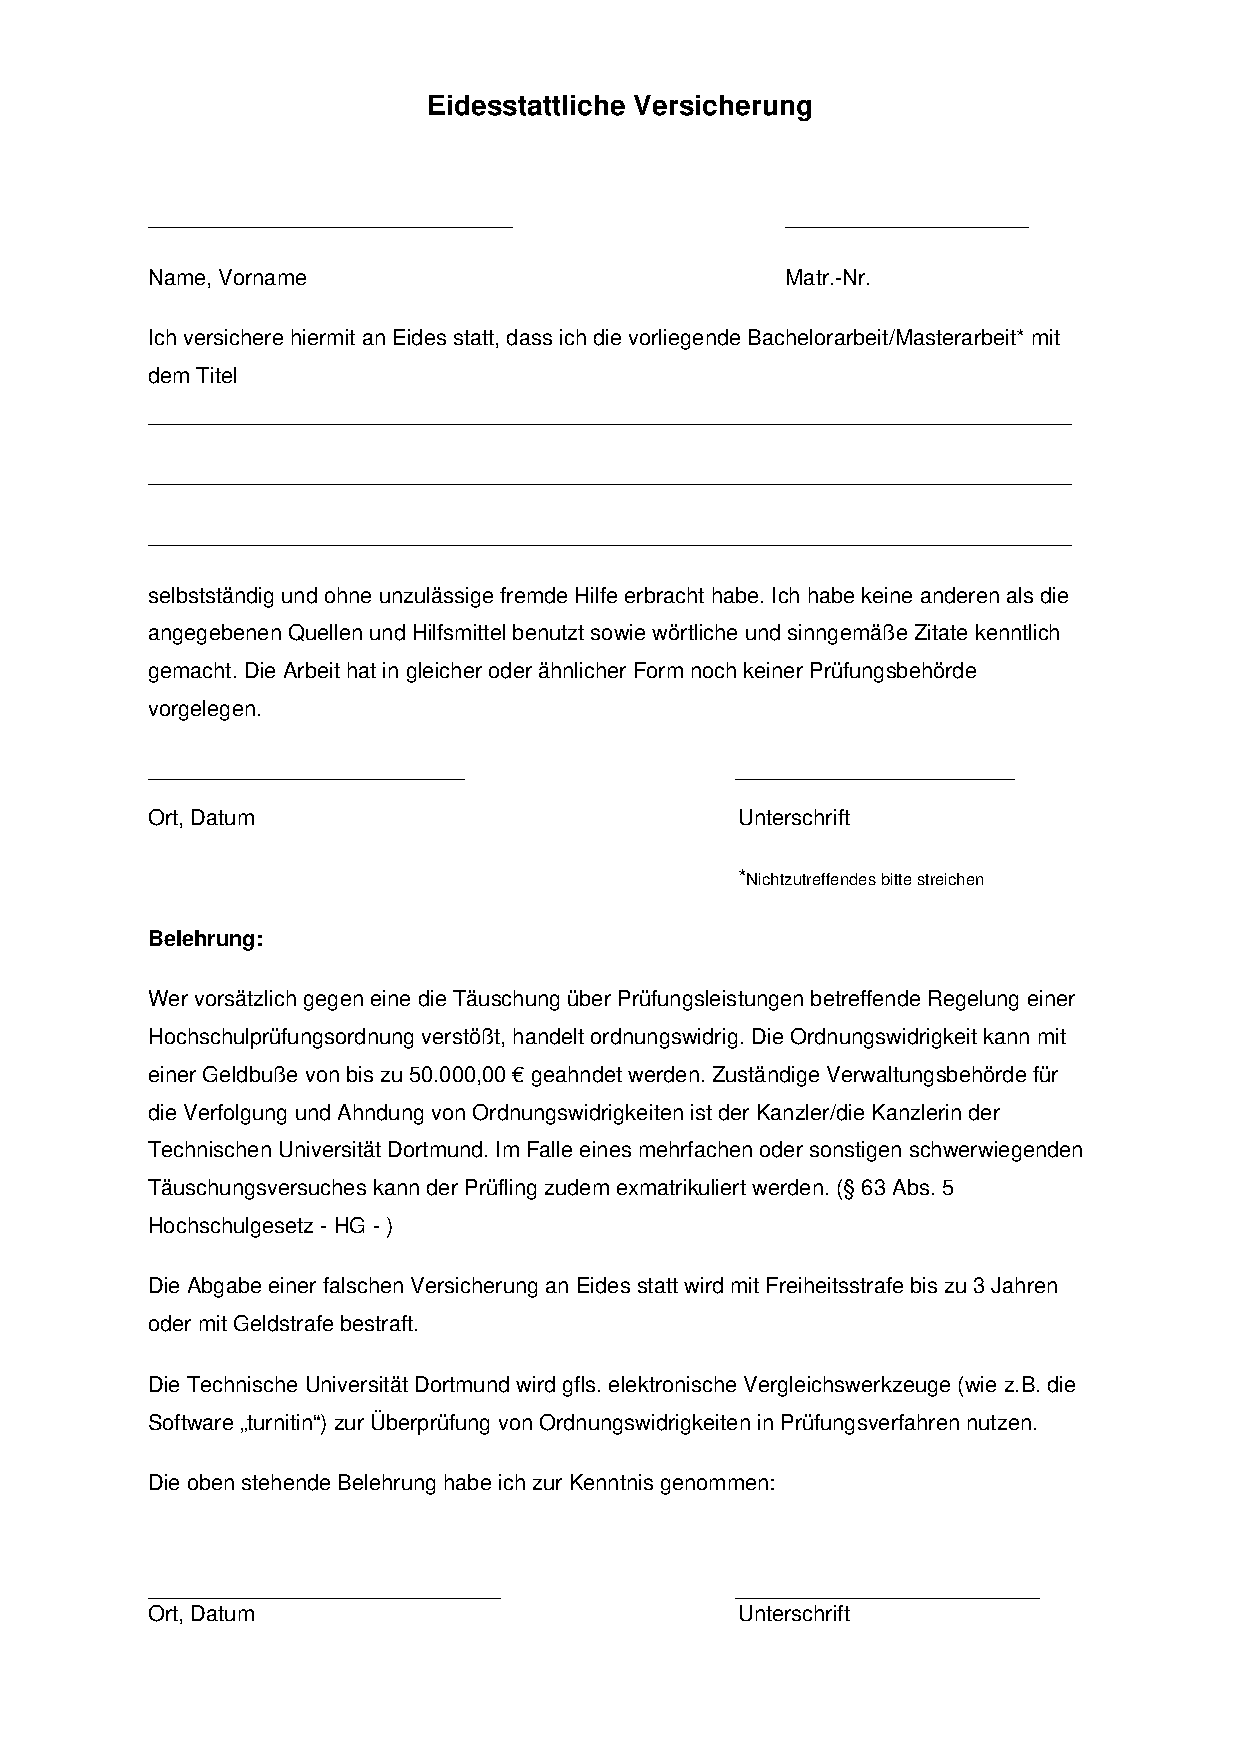
\includepdf{chapters/versicherung}

\end{document}
